\documentclass[a4paper,10pt]{article}

\usepackage[T1]{fontenc}
\usepackage{color, listings}

\lstset{language=[Sharp]C, % Grundsprache ist C und Dialekt ist Sharp (C#)
basicstyle=\small,
captionpos=b, % Beschriftung ist unterhalb
%frame=lines, % Oberhalb und unterhalb des Listings ist eine Linie
frame=rlub
basicstyle=\ttfamily, % Schriftart
keywordstyle=\color{blue}, % Farbe für die Keywords wie public, void, object u.s.w.
commentstyle=\color{green}, % Farbe der Kommentare
stringstyle=\color{red}, % Farbe der Zeichenketten
breaklines=true, % Wordwrap a.k.a. Zeilenumbruch aktiviert
showstringspaces=false, % emph legt Farben für bestimmte Wörter manuell fest
emph={double,bool,int,unsigned,char,true,false,void},
emphstyle=\color{blue},
emph={Assert,Test},
emphstyle=\color{red},
emph={[2]\using,\#define,\#ifdef,\#endif}, 
emphstyle={[2]\color{blue}}
}

%\renewcommand{\rmdefault}{ppl} %Palatino
%\renewcommand{\rmdefault}{cmfib} % computer modern fibonacci 365
%\renewcommand{\rmdefault}{\sfdefault} default serifenlos
\usepackage{ae}
\renewcommand{\familydefault}{phv} % Helvetica angenehm zu lesen ! 386
\usepackage{graphicx}

% Silbentrennung
\usepackage[english,ngerman]{babel}

% PDF
%LaTeX erzeugt mit dem hyperref-Paket interaktive PDF-Dateien mit Bookmarks
\usepackage{color}
\usepackage[colorlinks]{hyperref}
\usepackage{my} % modifizierte Ueberschriften
%\usepackage{avant}
%\usepackage{mathptmx}

%empfohlen aber gehen leider nicht:
%\usepackage{microtype} Optischer Randausgleich besserer Rand
%\usepackage{mparhack}


%Einstellungen der Seitenränder
% \usepackage[left=3cm,right=3cm,top=3cm,bottom=3cm,includeheadfoot]{geometry}

%Umlaute ermöglichen
\usepackage[latin1]{inputenc}
\usepackage{tabularx} % Seite 259 im Latex Buch, ist extrem cool !!
\newcolumntype{Y}{>{\small\raggedright\arraybackslash}X}


%Kopf- und Fußzeile
\usepackage{fancyhdr}
\pagestyle{fancy}
\fancyhf{}

%Kopfzeile mittig
\fancyhead[C]{\nouppercase{\leftmark}}
%Linie oben
\renewcommand{\headrulewidth}{0.5pt}

%Fußzeile mittig
\fancyfoot[C]{\thepage}
%Linie unten
\renewcommand{\footrulewidth}{0.5pt}

\selectlanguage{english} 



\begin{document}

{\sc Die Schriftart small caps (Kapit"alchen).}
{\sf Die Schriftart sans serif (serifenlos).}

\tableofcontents
\newpage

TODO:

Welchen typen unterstuetzen wir
Alle Ausdruecke werden bei uns in der Klasse Symboltable ueberprueft auf Korrektheit. 


\section{Parser}

The first set is very interesting for a top down parser. The parser compares the actual token with the first-sets symbol and takes decisions between alternatives. To guarantee that the decision between two alternatives is correct, the first set of the alternatives must be disjunctive. 

% TODO umschreiben (ANFANG)
%We defined the first-sets and follow-sets to check that we can really achieve that a lookahead of one symbol is sufficient.

%The first set very interesting for a top down analysis, because it determines the progress of the analysis.
%The first set of a node contains all token, by which the parser will be guided to the node.

%If the actual text isn't matched by one of the token of the first set, an other node will be chosen, namely the node with the first set that contains a token, which matches. If there is no such alternative the parsing is stopped with an error message. To guarantee that the decision between alternatives is definite, the first sets of the alternatives must be disjunctive, i.e.: there may not be a token contained in two alternative first sets. 

% TODO umschreiben (ENDE)

\subsection{First Sets}

% use packages: array
\begin{tabular}{p{4cm}l}
	S & First(S) \\ \hline
	& \\
	program & package\_declaration package\_import  \\
	package\_declaration & "package" \\
	package\_import & "import" \\
	class\_declaration & "public" \\
	class\_block & method\_declaration datatype\_declaration \\
	method\_declaration & "public" \\
	datatype\_declaration & "static" datatype\_decsriptor \\
	method\_call & identifier \\
	datatype\_assignment & identifier \\
	body\_block & while\_statement if\_statement return\_statement datatype\_declaration identifier (method\_call datatype\_assignment) \\
	while\_statement & "while" \\
	if\_statement & "if" \\
	return\_statement & "return" \\
	datatype\_decsriptor & datatype \\
	datatype & primitive object \\
	primitive & "int" "boolean" "char" \\
	object & String identifier \\
	identifier & letter \\
	selector & "." "[" \\
	condition & expression \\
	expression & term \\
	term & factor \\
	factor & value \\
	value & identifier datatype not\_value TODO \\
	integer & "-" digit\_non\_zero \\
	char & "'"\\
	boolean & "true" "false" \\
	string & """ \\
	digit & digit\_non\_zero digit\_zero \\
	digit\_non\_zero & 1 2 3 4 5 6 7 8 9 \\
	digit\_zero & 0 \\
\end{tabular}


\begin{figure}
	\begin{center}
	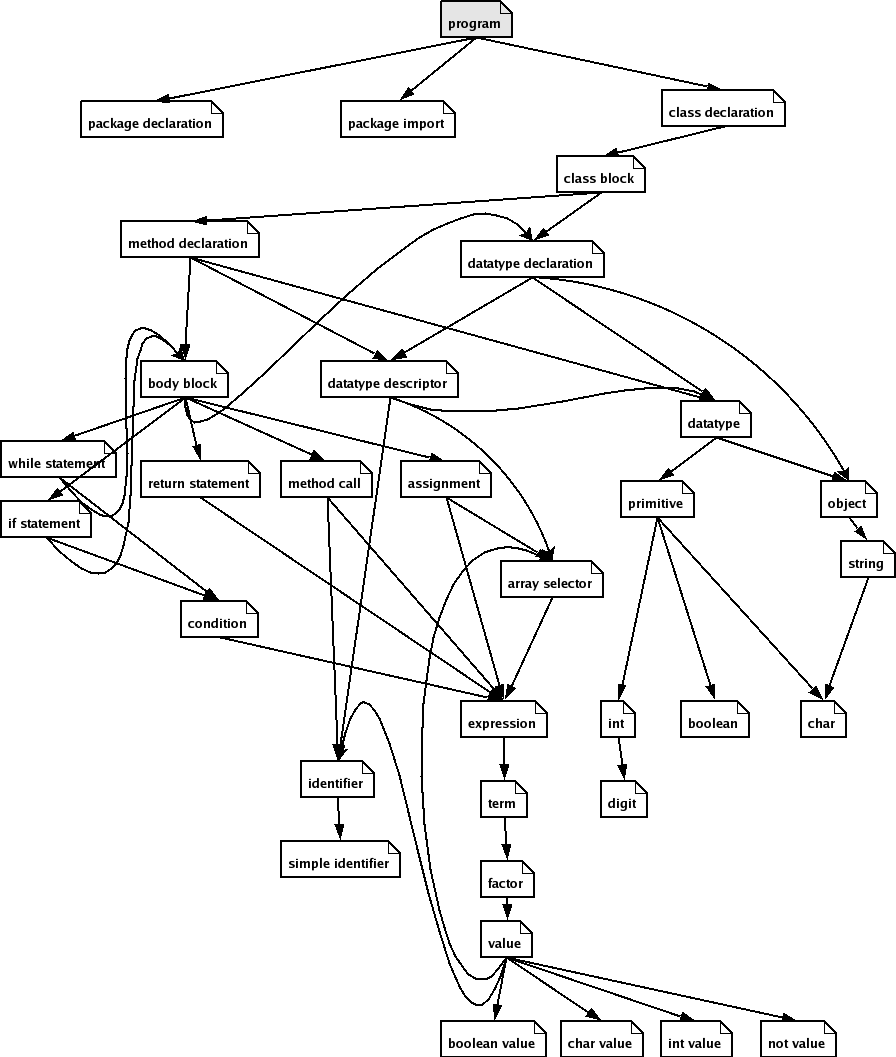
\includegraphics[scale=0.4]{Diagram_Small.png}
% Diagram_Small.eps: 300dpi, width=10.83cm, height=12.67cm, bb=0 0 1279 1497 ,bb=0 0 1279 1497
% width=15cm,height=15cm
	
	\label{dep_diagram}
	\caption {Dependencies representation of parsing procedures (simplified).}
	\end{center}
\end{figure}

\section{Memorymanagement in comPiler}
ComPiler compiles code for RISC-based architectures. It has 32 registers each
with size 32 Bit (4 Byte). Register 0 (R0) has always the value 0. Register 31
(R31) is reserved for return addresses. In a branch instruction the PC is stored
in R31. 

The instruction register (IR) holds the current instruction being executed. \newline 
The program counter (PC) contains the address of the instruction to be
fetched next. \newline
The stack pointer (SP) indicates the top element of a register-based stack. That
means that on some occasions registers are accessed like a stack and the SP
points out the next free register.  
\newline
The memory for the activation frames is organized like a stack. Each frame is an
entry. The SP indicates the next free memory and the FP the base address of the
current frame. 
\subsubsection{Organization of an activation frame}
An activation frame is a special memory context used for a procedure and its
local variables. It's created by a branch instruction (e.g. a procedure call). The base address of the activation 
frame is also the base address for all local variables declared here. Because this base address is highly 
important and one needs to access it efficently it's saved in the frame pointer (FP).
As the former PC was saved at the branch instruction, we use it as our return
address and save it in R31.



\subsection{local variables}
ComPiler offers local hiding of variables. That means, that procedures can
contain variables that cannot be seen outside the procedure. Even if there
exists a variable with the same name outside the procedure, these two don't
interfere. 
\subsubsection*{So what happens when a branch instruction occurs?}
When the instruction is executed, the PC is stored in R31. Then the code
generator jumps to the next instruction-address indicated by the branch instruction.
Now we have entered a special memory context for procedures (an activation frame). In this frame all memory is 
managed that is needed in the procedure
\newline
  
 


Local variables have the following properties: 
\begin{itemize}
  \item They have negative offsets to their baseaddresses
\end{itemize}



\section{The symbolfile}
The symbolfile (file-extension is .sym)is a sequential representation of the
symboltable. All entries
are representations of the symbols found in the sourcecode. \\
Because the symbolfile is just read one time during compilation, it cannot be
seen as a performance factor. So we decided to write the symbolfile in
xml-format as it is a good representation of objects. 
\subsection{Structure}
The root-tag of the symbolfile is \emph{<symbolfile>}. After the xml-header and
the root-tag the symbolfile starts with a list of the so-called \emph{module anchors}. Every
module anchor represents a module that's imported. In xml-syntax this lookes
like that:
\begin{lstlisting}[caption={module anchors}]
<modules>
	<module>
		<name> modulename 1 </name>
	</module>
	<module>
		<name> modulename 2 </name>
	</module>
	<module>
		<name> modulename 3 </name>
	</module>
</modules>
\end{lstlisting}

After the module anchors the actual symboltable representation starts. It is
enclosed in a \emph{<symbols>}-tag There are 3 different elementtypes that can be described here:
\begin{itemize}
  \item variables
  \item arrays
  \item methods 
\end{itemize}
\subsubsection{variables}
A variable has 2 properties: 
\begin{itemize}
  \item one of the primitive datatypes like \emph{boolean}, \emph{int} or \emph{char}
  \item the name of the variable in the sourcecode
\end{itemize}

\begin{lstlisting}[caption={variables}]
<variable>
	<type> type </type>
	<name> name </name>
</variable>
\end{lstlisting}

\subsubsection{arrays}
An array has 3 properties
\begin{itemize}
  \item one of the primitive datatypes like \emph{boolean}, \emph{int} or \emph{char}
  \item the name of the variable in the sourcecode
  \item the number of elements in the array
\end{itemize}

\begin{lstlisting}[caption={arrays}]
<array>
	<type> type </type>
	<name> name </name>
	<size> size </size>
</array>
\end{lstlisting}

\subsubsection{methods}
An array has 3 properties and contains another symboltable with the parameters
of the method. 
\begin{itemize}
  \item the return value of the method as one of the primitive datatypes
  like \emph{boolean}, \emph{int} or \emph{char}
  \item the name of the method in the sourcecode
  \item the number of elements in the array
\end{itemize}
So the description of a method is a recursive search through the symboltable.

\begin{lstlisting}[caption={methods}]
<method>
	<type> type </type>
	<name> name </name>
	<size> size </size>
	<symbols>
		<variable>
			<type> type </type>
			<name> name </name>
		<variable>
	</symbols>
</method>
\end{lstlisting}

\part{The linker}
The linker is a intermediate step between processing the sourcecode and executing a
binary. It reads the objectfiles of a compiled program and its imported
modules and combines them to one binary for the virtual machine.
\\
A linker is needed if a compiler wants to provide \emph{separate compilation}.
That means that a program can import methods from a precompiled module. The
program just needs a symbolfile to find out which methods the module offers. \\
But a problem arises when the compiler wants to create a binary from the
program-sourcecode. The compiler knows that the called method exists in the
module (from the symbolfile) but it doesn't know the content of that method. \\
So before the program can be executed the linker has to copy the relevant data
from the affected objectfiles together into one binary. These objectfiles contain
all the information the linker needs to fullfill that work.    

\section{The objectfile}
\label{objectfile}
The objectfile is a intermediate file created by the compiler, that already
contains generated code and a lot of meta-information. The linker reads this
objectfile and creates a binaryfile. \\
The reason for that intermediate step is, that if modules are imported the
compiler doesn't have all the data he needs to create a valid and executable binary. 
So the objectfile offers the needed information like the program entry point, which
methods are loaded from modules and were to find that methods in these modules. \\
Based in that information the linker can link the compiled code in the
objectfiles together and create one executable binary.

\subsection{Structure}
\label{linker:objectfile:structure}
The structure of an objectfile is quite simple as one can see below. Its basic
datasize is 32 bit. That means all data except character are represented and 
stored as 32 bit integers. A character is a 1-byte-value (8-bit). \\
\begin{figure}[h]
	\begin{center}
	
		\begin{tabular}{|c|}
			\hline
			magic word \\
			\hline 
			branch instruction to main method \\
			\hline
			lenght of offset table \\
			\hline
			offset table \\ \\
			\hline
			lenght of fixup table \\
			\hline
			fixup table \\ \\
			\hline
			opCode \\ \\
			\hline 
		\end{tabular}
	
	\end{center}

\caption{structure of an objectfile}
\label{linker:objectfile:example:structure}

\end{figure} 

\subsubsection{magic word} 
\label{linker:objectfile:magic_word}
The magic word identifies the objectfile. Its value has to be $0$ represented
by a 32 bit integer value. 
\subsubsection{branch instruction to main method}
\label{linker:objectfile:branch_to_main}
This is an integer-representation of the branch-instruction to the address of
the main-method in this objectfile. 
\subsubsection{length of the offset table}
\label{linker:objectfile:length_offset_table}
The length of the offset table as a 32 bit integer value. The unit of this value
is one 32 bit word. 
\subsubsection{offset table}
\label{linker:objectfile:offset_table}
In the offset table variable- or methodnames and their offsets in the current
module are saved. That means that every exported module element stands in the
offset table with its name and opCode offset in the modulefile.  \\
The example in ~\ref{linker:objectfile:example:offset_table} shows the method
\emph{print}:

\begin{figure}[h]
	\begin{center}
		\begin{tabular}{|c|c|c|c|}
			\hline
			P &  R & I & N \\
			\hline
			T &  = &  0 & 0 \\
			\hline 
			\multicolumn{4}{|c|}{value} \\
			\hline
			\multicolumn{4}{|c|}{\ldots} \\
			\hline
		\end{tabular}
	\end{center}
	\caption{offset table}
	\label{linker:objectfile:example:offset_table}
\end{figure}

The bytes until the equal-sign form the name of the symbol. The next bytes
are skipped so that only complete 32 bit words are read (in our example 2 bytes). 
The next 32 bit word is the offset of the instruction (opCode) for access to that 
element in the module. The length of the offset table (~\ref{linker:objectfile:length_offset_table})  
defines how often this operations are performed. 

\subsubsection{length of the fixup table}
\label{linker:objectfile:length_fixup_table}
The length of the fixup table as a 32 bit integer value. The unit of this value
is one 32 bit word. 
\subsubsection{fixup table}
\label{linker:objectfile:fixup_table}
In the fixup table the local and imported methods (methods from other modules) are
listed. That means their modulename, their name and their offset in the module are stored. \\
The example in ~\ref{linker:objectfile:example:fixup_table} shows a fixup table
with the \emph{print}-method from the module \emph{Util}.

\begin{figure}[h]
		
	\begin{center}
		\begin{tabular}{|c|c|c|c|}
			\hline
			U & T & I & L \\
			\hline
			. & P & R & I \\
			\hline
			N & T & = & 0 \\
			\hline 
			\multicolumn{4}{|c|}{value} \\
			\hline
			\multicolumn{4}{|c|}{\ldots} \\
			\hline
		\end{tabular}
	\end{center}
	
	\caption{fixup table}
	\label{linker:objectfile:example:fixup_table}
\end{figure}
The bytes from the beginning to the first dot form the modulename. The following
bytes to the equals-sign form the symbolname. The next bytes (in our example one
byte) are skipped so that only 32 bit words are read. \\
This reading-operation is performed until the number of words in the length of
the fixup table (~\ref{linker:objectfile:length_fixup_table}) is read.

\subsection{Processing of the objectfiles}
\label{linker:objectfile_procession}
As mentioned above the linker combines one or more objectfiles to one binary for
execution in the virtual machine.\\ 

\begin{figure}[h]

\begin{tabular}{c c}

		\begin{tabular}{|c|}
			\hline
			0 \\
			\hline 
			0 \\
			\hline
			0 \\
			\hline
			\\ \\ \\ \\ \\ \\
			\hline
			4 \\
			\hline
			% the fixup table
			\begin{tabular}{|c|c|c|c|}
				U & T & I & L \\
				\hline
				. & P & R & I \\
				\hline
				N & T & = & 0 \\
				\hline 
				\multicolumn{4}{|c|}{18} \\
			\end{tabular}
			% ! the fixup table
			\\
			\hline
			% the opCode
			\begin{tabular}{c}
				$ \cdots $ \\
				\hline
				line 18: method call for Util.print \\
				\hline
				$ \cdots $ \\
			\end{tabular}
			% ! the opCode
			\\
			\hline 
		\end{tabular}

		\begin{tabular}{|c|}
			\hline
			0 \\
			\hline 
			0 \\
			\hline
			6 \\
			\hline
			% offset table
			\begin{tabular}{|c|c|c|c|}
				P & R & I & N \\
				\hline
				T &  = &  0 & 0 \\
				\hline 
				\multicolumn{4}{|c|}{23} \\
				\hline
				C & A & L & C \\
				\hline
				= &  0 &  0 & 0 \\
				\hline 
				\multicolumn{4}{|c|}{42} \\
			\end{tabular}
			% ! offset table
			\\ 
			\hline
			0 \\
			\hline
			\\ \\ \\ \\
			\hline
			% the opCode
			\begin{tabular}{c}
				$ \cdots $ \\
				\hline
				line 23: entry point of method print \\
				\hline
				$ \cdots $ \\
			\end{tabular}
			% ! the opCode
			\\
			\hline 
		\end{tabular}

\end{tabular}
\caption{The objectfile of the main-module and the util-module}
\label{linker:example:linker}
\end{figure}

The example in ~\ref{linker:example:linker} shows what data the linker reads from the
objectfiles and how this data is processed. \\
The fixup table is the key element in linking. It points out that code
instructions which need to be fixed (their jump addresses must be corrected).
In the example the instruction at position 18 in the opCode must be corrected. \\
These jump addresses can be read from the offset table. If an entry in the fixup
table points to another module the offset table of that particular module
provides that information.  \\
In the example the offset table shows that the instruction at position 23 in the
opCode of \emph{Util} is the target address for the jump instruction in the
fixup table. \\
\\
The values the offset table provides are relative to their module. That means
that in module \emph{Util} the entry point for the \emph{print}-instruction is
at position 23 in the opCode. But if this objectfile is linked to another
objectfile this opCode is appended to the opCode of the other objectFile. So
these relative positions change. \\
The linker takes care of this addressing inconsistency. It updates the offset
table when a module is linked to another one. 


\section{The binaryfile}
The binaryfile is a file that can be executed by the virtual machine. It hardly
provides any meta-information but mostly executable code (opCode). This file is
created when a linker links one or more objectfiles together. \\
Linking means that the opCode from the objectfiles is copied sequentially into the
binaryfile and that jump addresses in this opCode are corrected. 

\subsection{Structure}
The binary file always starts with a magic word of length 32 bit, so that the
virtual machine can identify it as an executable. The magic word always has the value 0.
\\ \begin{figure}[h]
		
	\begin{center}
		\begin{tabular}{|c|c|c|c|}
			\hline
				magic word (32 bit) \\
			\hline
				opCode of the main module \\	
			\hline
				$\cdots$ \\
			\hline
				exit instruction \\
			\hline
			opCode of the first imported module \\	
			\hline
				$\cdots$ \\
			\hline
			opCode of the second imported module \\	
			\hline
				$\cdots$ \\
			\hline
		\end{tabular}
	\end{center}
	
	\caption{Structure of the binary file}
	\label{linker:binaryfile:structure}
\end{figure}
After the magic word the opCode instructions of the main module are stored
followed by an exit instruction (jump to address (-1)). If the virtual machine
reads this instruction, it stops execution. \\
The following content are the instructions of the imported modules in the order
they were imported by the main module (importing means, that one of their
methods was called).


\end{document}
